\documentclass[12pt]{article}

% Packages
\usepackage{amsmath, amssymb}
\usepackage{graphicx}
\usepackage{booktabs}
\usepackage{subcaption}
\usepackage{hyperref}
\usepackage{geometry}
\usepackage{minted}   % requires: pdflatex -shell-escape
\geometry{margin=1in}

\title{Machine-Learning Based Encryption via Learned Character Permutations}
\author{Samuel Cavazos}
\date{\today}

\begin{document}

\maketitle

\begin{abstract}
A cipher is covered early on in elementary cryptography courses because it provides intuition about more complicated encryption methods. In this paper, we implement a random substitution cipher in Python and train two neural networks to learn the mapping. The models, implemented in PyTorch, serve as an \textbf{encoder} (plaintext $\rightarrow$ ciphertext) and a \textbf{decoder} (ciphertext $\rightarrow$ plaintext). Together, they demonstrate how machine learning can memorize and reproduce encryption and decryption operations for a fixed, randomly sampled key (permutation) over a finite character vocabulary. While we begin with this simple cipher, the flexibility of neural models enables more sophisticated approaches—for example, using learnable \emph{embeddings} to represent symbols as vectors and composing them with richer architectures which allows for the possibility of more complicated and secure encryption methods.
\end{abstract}

\section{Problem Setup and Notation}
Let $V$ denote a finite character vocabulary with $|V|=n$. We index symbols by integers $\{0,1,\dots,n-1\}$ and write $\pi\in S_n$ for a key sampled uniformly at random: $\pi:\{0,\dots,n-1\}\!\to\!\{0,\dots,n-1\}$ is a permutation. The \emph{encryption} function is $E_\pi(i)=\pi(i)$ and the \emph{decryption} function is $D_\pi(j)=\pi^{-1}(j)$.

We cast learning $E_\pi$ and $D_\pi$ as two multi-class classification problems over $n$ classes. The supervised pairs are
\[
\mathcal{D}_{\mathrm{enc}}=\{(x,\pi(x))\,:\,x\in\{0,\dots,n-1\}\},\qquad
\mathcal{D}_{\mathrm{dec}}=\{(\pi(x),x)\,:\,x\in\{0,\dots,n-1\}\}.
\]

\paragraph{One-hot and embeddings.}
Let $e_i\in\mathbb{R}^n$ denote the $i$-th standard basis vector. We will use a learnable embedding $E\in\mathbb{R}^{n\times d}$ that maps index $i$ to $E^\top e_i\in\mathbb{R}^d$ (equivalently, the $i$-th row of $E$).

\section{Model Architecture}
For each direction we use the same per-character classifier. Given input index $x\in\{0,\dots,n-1\}$, the model computes
\begin{align}
\text{Embedding: } & \quad h = E^\top e_x \in \mathbb{R}^d, \\
\text{Logits: } & \quad z = W h + b \in \mathbb{R}^{n}, \\
\text{Class probs: } & \quad p(y\,|\,x) = \mathrm{softmax}(z)_y = \frac{\exp(z_y)}{\sum_{k=0}^{n-1}\exp(z_k)},
\end{align}
with parameters $E\in\mathbb{R}^{n\times d}$, $W\in\mathbb{R}^{n\times d}$, $b\in\mathbb{R}^{n}$. The prediction is $\hat{y}=\arg\max_y p(y\,|\,x)$.

\paragraph{Expressivity (exact realization).}
\textbf{Proposition.} If $d\ge n$, there exist parameters $(E,W,b)$ such that $\arg\max \mathrm{softmax}(W E^\top e_x + b) = \pi(x)$ for all $x$. In particular, choose $E=I_n$, $b=0$, and $W=P_\pi$, the permutation matrix corresponding to $\pi$ (i.e., $(P_\pi)_{y,x}=1$ iff $y=\pi(x)$). Then $W E^\top e_x = P_\pi e_x = e_{\pi(x)}$, and the softmax is maximized uniquely at class $\pi(x)$.

This guarantees that a shallow embedding+linear model can perfectly implement any substitution cipher when $d\!\ge\!n$; in practice we use $d\ll n$ and still find the mapping by optimization.

\section{Learning Objective}
For either direction (encoder or decoder) with dataset $\mathcal{D}=\{(x_i,y_i)\}_{i=1}^N$, the negative log-likelihood (cross-entropy) is
\begin{equation}
\mathcal{L}(\theta) \;=\; -\frac{1}{N}\sum_{i=1}^{N}\log p_\theta(y_i\,|\,x_i)
\;=\; -\frac{1}{N}\sum_{i=1}^{N}\Big(z_{i,y_i} - \log\sum_{k=0}^{n-1} e^{z_{i,k}}\Big),
\end{equation}
where $z_i=W E^\top e_{x_i}+b$ are the logits for example $i$ and $\theta=(E,W,b)$. We optimize with Adam. Accuracy is $\tfrac{1}{N}\sum_i \mathbf{1}\{\arg\max_k z_{i,k}=y_i\}$.

\paragraph{Computational notes.}
Per example, the forward pass costs $O(dn)$ to produce logits (matrix-vector multiply $W h$), and the softmax normalization costs $O(n)$. Thus the softmax dimension $n=|V|$ dominates compute and memory, motivating an ASCII-sized vocabulary in our initial experiments.

\section{Implementation (Minimal, Self-Contained)}
We present compact Python listings that realize the mathematics.

\subsection{Vocabulary}
We fix $V$ by concatenating ASCII letters, digits, punctuation, and whitespace, and provide index$\leftrightarrow$character utilities.
\begin{minted}[fontsize=\footnotesize, frame=single]{python}
import string, torch

class Characters:
    def __init__(self):
        self.characters = (
            string.ascii_letters + 
            string.digits + 
            string.punctuation + 
            " \t\n\r\x0b\x0c"
        )
        self.num_characters = len(self.characters)
    def index(self, text: str) -> torch.Tensor:
        return torch.tensor([self.characters.index(c) for c in text], dtype=torch.long)
    def read(self, indices: torch.Tensor) -> str:
        return "".join(self.characters[int(i)] for i in indices)
\end{minted}

\subsection{Random substitution supervision}
We sample $\pi$ and build paired supervision for $E_\pi$ and $D_\pi$.
\[
\mathcal{D}_{\text{enc}}=\{(x,\pi(x))\},\qquad
\mathcal{D}_{\text{dec}}=\{(\pi(x),x)\}.
\]
\begin{minted}[fontsize=\footnotesize, frame=single]{python}
import random, torch

class Cipher:
    def __init__(self):
        self.char = Characters()
        n = self.char.num_characters
        self.pi = list(range(n)); random.shuffle(self.pi)
        # paired tensors: (src, dst)
        self.enc_pairs = torch.tensor([range(n), self.pi], dtype=torch.long).T
        self.dec_pairs = torch.tensor([self.pi, range(n)], dtype=torch.long).T

cipher = Cipher()
\end{minted}

\subsection{Architecture (Embedding $\to$ Linear)}
This implements $h=E^\top e_x$, $z=Wh+b$, $p=\mathrm{softmax}(z)$.
\begin{minted}[fontsize=\footnotesize, frame=single]{python}
import torch.nn as nn

class Architecture(nn.Module):
    def __init__(self, num_chars: int, emb_dim: int = 64):
        super().__init__()
        self.emb = nn.Embedding(num_chars, emb_dim)  # rows = E
        self.out = nn.Linear(emb_dim, num_chars)     # W, b
    def forward(self, x):                            # x: [B]
        return self.out(self.emb(x))                 # logits: [B, |V|]
\end{minted}

\subsection{Training loop (encoder and decoder)}
Two instances of the same architecture are trained on the two directions.
\begin{minted}[fontsize=\footnotesize, frame=single]{python}
import torch, torch.utils.data as data

V = cipher.char.num_characters
encoder, decoder = Architecture(V), Architecture(V)
criterion = nn.CrossEntropyLoss()
enc_opt = torch.optim.Adam(encoder.parameters(), lr=2e-3)
dec_opt = torch.optim.Adam(decoder.parameters(), lr=2e-3)

# datasets of (x, y) indices
enc_ds = data.TensorDataset(cipher.enc_pairs[:,0], cipher.enc_pairs[:,1])
dec_ds = data.TensorDataset(cipher.dec_pairs[:,0], cipher.dec_pairs[:,1])
enc_loader = data.DataLoader(enc_ds, batch_size=32, shuffle=True)
dec_loader = data.DataLoader(dec_ds, batch_size=32, shuffle=True)

@torch.no_grad()
def eval_mapper(model, pairs):
    x, y = pairs[:,0], pairs[:,1]
    logits = model(x)
    loss = criterion(logits, y).item()
    acc = (logits.argmax(-1) == y).float().mean().item()
    return loss, acc

for epoch in range(1, 501):
    # encoder step
    encoder.train()
    for x, y in enc_loader:
        enc_opt.zero_grad(set_to_none=True)
        loss = criterion(encoder(x), y)
        loss.backward(); enc_opt.step()
    # decoder step
    decoder.train()
    for x, y in dec_loader:
        dec_opt.zero_grad(set_to_none=True)
        loss = criterion(decoder(x), y)
        loss.backward(); dec_opt.step()
    # evaluation on all symbols
    enc_loss, enc_acc = eval_mapper(encoder, cipher.enc_pairs)
    dec_loss, dec_acc = eval_mapper(decoder, cipher.dec_pairs)

    if enc_acc == 1.0 and dec_acc == 1.0:
        torch.save(encoder.state_dict(), "encoder.pth")
        torch.save(decoder.state_dict(), "decoder.pth")
        print("Training complete."); break
\end{minted}

\section{Results}
On an ASCII-sized vocabulary, both models rapidly achieve $100\%$ accuracy on their respective mappings, demonstrating that the embedding+linear architecture can memorize and invert a random permutation of $V$.

\subsection*{Experimental Protocol for Figures}
To quantify learning speed and variability, we run a sweep of $T$ independent trainings (e.g., $T=1000$), each with a fresh random permutation $\pi$ and fixed hyperparameters (batch size $32$, embedding dimension $64$, learning rate $2\times10^{-3}$, maximum epochs $300$). For each run we log per-epoch metrics and define the \emph{epochs-to-convergence}
\[
\tau \;=\; \min\{\,e\in\mathbb{N} \;|\; \texttt{enc\_acc}_e \ge 1.0 \ \wedge\  \texttt{dec\_acc}_e \ge 1.0 \,\}.
\]
Aggregate training curves compute, for each epoch $e$, the median and interquartile range (IQR, $25$--$75$th percentile) across all trials that reached epoch $e$. Wall-clock time is measured per run with a simple start/stop timer.

\begin{figure}[h]
    \centering
    \begin{minipage}[t]{0.48\textwidth}
        \centering
        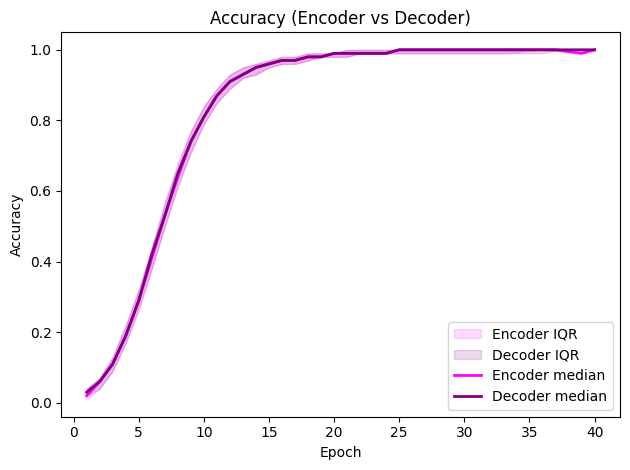
\includegraphics[width=\textwidth]{accuracy.png}
        \caption{\textbf{Accuracy (median \& IQR).} Encoder (magenta) vs.\ decoder (purple). Shaded bands indicate IQR across trials; solid curves are medians. The two curves nearly overlap, reflecting symmetry of the forward and inverse mappings.}
        \label{fig:acc-curves}
    \end{minipage}
    \hfill
    \begin{minipage}[t]{0.48\textwidth}
        \centering
        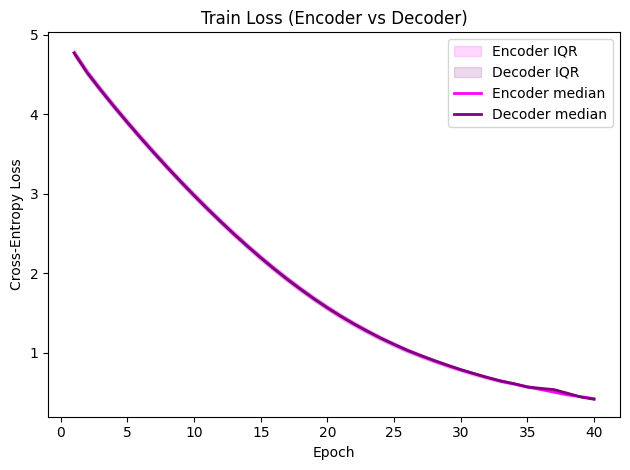
\includegraphics[width=\textwidth]{train_loss.png}
        \caption{\textbf{Train loss (median \& IQR).} Cross-entropy loss for encoder (magenta) and decoder (purple). Loss decays smoothly to near-zero as the permutation is memorized.}
        \label{fig:loss-curves}
    \end{minipage}
\end{figure}

\begin{figure}[t]
    \centering
    \begin{subfigure}{0.49\textwidth}
        \centering
        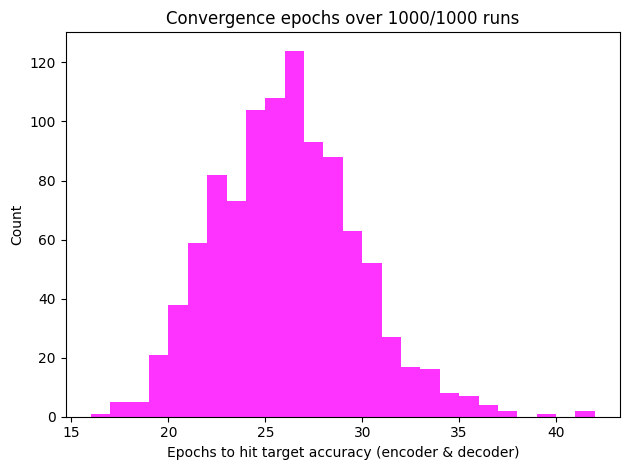
\includegraphics[width=\linewidth]{convergence_epochs.png}
        \caption{\textbf{Epochs to convergence.} Histogram of $\tau$ across runs. Mass concentrates in the low tens of epochs, consistent with rapid memorization of a finite permutation.}
        \label{fig:epochs-conv}
    \end{subfigure}
    \hfill
    \begin{subfigure}{0.49\textwidth}
        \centering
        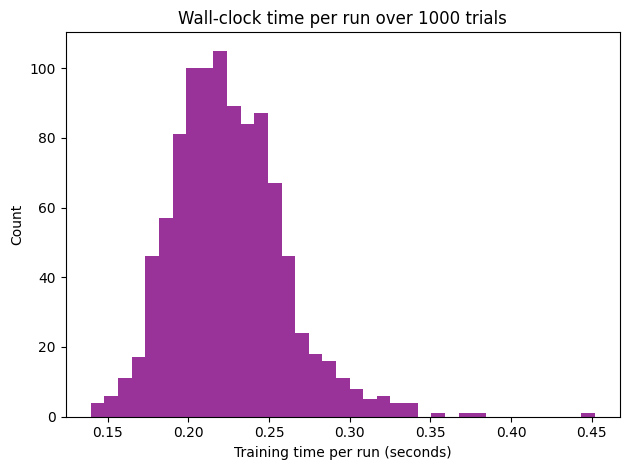
\includegraphics[width=\linewidth]{time-distribution.png}
        \caption{\textbf{Wall-clock time per run.} Distribution of end-to-end training time (seconds) for one encoder/decoder pair on the given hardware.}
        \label{fig:time-dist}
    \end{subfigure}
    \caption{\textbf{Convergence behavior over many independent trainings.} Left: how many epochs until both models reach $100\%$ accuracy. Right: elapsed time per run.}
    \label{fig:convergence-summary}
\end{figure}

\section{Discussion}
The experiment isolates the mathematical core of learned substitution: logits $z=Wh+b$ over $n$ classes, a cross-entropy objective, and a small embedding dimension $d$. The proposition shows exact realizability when $d\ge n$; empirically, $d\ll n$ suffices in practice for this finite task. The aggregated curves in Figures~\ref{fig:acc-curves}--\ref{fig:loss-curves} show fast, stable convergence, while Figure~\ref{fig:convergence-summary} summarizes the distribution of required epochs and wall-clock time across random keys.

\paragraph{Security note (single mention).} This study examines mechanics of learned mappings and is not intended as a cryptosystem.

\section{Toward Richer Settings}
Two directions naturally follow:
\begin{itemize}
    \item \textbf{Scaling $|V|$.} Moving beyond ASCII toward UTF encodings increases the softmax dimension and compute; subword vocabularies or hierarchical classifiers may mitigate the $O(n)$ normalization cost.
    \item \textbf{Sequence conditioning.} Replace per-character substitution with key-conditioned sequence models; analyze behavior under chosen-plaintext/ciphertext regimes and investigate integrity constraints.
\end{itemize}

\section{Code and Installation}
The full source code for this project is available at:
\href{https://github.com/Alshivals-Data-Service/alshicrypt}{\texttt{github.com/Alshivals-Data-Service/alshicrypt}}.

\paragraph{Install (from GitHub).}
Requires Python 3.9+ and PyTorch 2.0+.
\begin{minted}[fontsize=\footnotesize]{bash}
pip install "git+https://github.com/Alshivals-Data-Service/alshicrypt.git"
# (If PyTorch is missing, install a wheel appropriate for your system first:
# https://pytorch.org/get-started/locally/)
\end{minted}

\paragraph{Quick start (train, save, load, use).}
\begin{minted}[fontsize=\footnotesize, frame=single]{python}
import alshicrypt

# Train & save to stable folders (each call samples a new random key)
crypt1 = alshicrypt.generate(epochs=200, outdir="artifacts/crypt-hello")
crypt2 = alshicrypt.generate(epochs=200, outdir="artifacts/crypt-world")

# Load them later (or in a new process)
crypt1 = alshicrypt.load("artifacts/crypt-hello")
crypt2 = alshicrypt.load("artifacts/crypt-world")

msg = "Hello, World!"
enc = crypt1.encode(msg)
dec = crypt1.decode(enc)
print("crypt1")
print("============================")
print(f"Original: {msg}")
print(f"Encoded:  {enc}")
print(f"Decoded:  {dec}\n")
assert dec == msg

enc2 = crypt2.encode(msg)
dec2 = crypt2.decode(enc2)
print("crypt2")
print("============================")
print(f"Original: {msg}")
print(f"Encoded:  {enc2}")
print(f"Decoded:  {dec2}")
assert dec2 == msg
\end{minted}

\begin{minted}[fontsize=\footnotesize]{text}
crypt1
============================
Original: Hello, World!
Encoded:  D<~~rJB*r)~W]
Decoded:  Hello, World!


crypt2
============================
Original: Hello, World!
Encoded:  d!VVm\x0b`Nm4V|-
Decoded:  Hello, World!
\end{minted}
\noindent Each trained pair is stored under the specified \texttt{artifacts/} directory
(e.g., \texttt{artifacts/crypt-hello}). The \texttt{encode} method applies the learned
plaintext$\rightarrow$ciphertext mapping; \texttt{decode} applies the inverse mapping.
Characters outside the training vocabulary are passed through unchanged.

\end{document}
